\chapter{\IfLanguageName{dutch}{Stand van zaken}{State of the art}}%
\label{ch:stand-van-zaken}

In dit onderdeel wordt dieper ingegaan op wat flutter is hoe het werkt. Daarna wordt er onderzocht welke state management benaderingen er 
zijn en hoe ze werken en worden ze met elkaar vergeleken.

\section{{Flutter}}%
\label{sec:Flutter}
Flutter is een open-source framework ontwikkeld door Google voor het bouwen van multi-platform applicaties vanuit één codebase. 
Dit betekent dus dat ontwikkelaars in een korte tijd applicaties kunnen ontwikkelen voor mobile, web, desktop en ook voor embedded systemen.
Bovendien wordt flutter code vertaald naar native machine code, wat zorgt voor snelle applicaties en annimaties. \footnote{\url{https://flutter.dev}}
\\
\\
Flutter applicaties worden geschreven met Dart, een programmeertaal die ook eigendom is van Google. Dart ondersteunt AOT (ahead of time) 
compilation en JIT (just in time) compilation. AOT verbetert de opstarttijd en performantie van de application en dankzij JIT compilation 
wordt hot reload mogelijk. Dit wilt zeggen dat enkel de gewijzigd stukken code opnieuw moet gecompileerd worden in plaats van de volledige applicatie.
Het is m.a.w. mogelijk om wijzigingen in bijna real time te testen. \footnote{\url{https://docs.dart.dev}}

\section{Flutter Architectuur}
\label{sec:Flutter Architectuur}
Voordat er over state management binnen flutter besproken kan worden, wordt er eerst een paar begrippen uitgelegd binnen Flutter. Ook wordt er in dit deel uitgelegd hoe Flutter werkt intern.

\subsection[widget]{Widgets}
\label{sec:Widgets}
In Flutter wordt alle componenten in een app als een "Widget" beschouwd. Wat een widget is, is eigenlijk een Dart-klasse die beschrijft hoe een stuk van de user interface eruitziet.
De UI van de app wordt m.a.w. gebouwd door widgets in ouder-kind relatie te combineren. Elk widget wordt in een parent widget genest en kan context doorgeven van ouder naar kind.
Als gevolg hiervan zitten alle widgets in een widgetboom, waarbij elk ouderwidget één of meerdere kind widgets kan hebben.
\\
\begin{figure}[h]
    \centering
    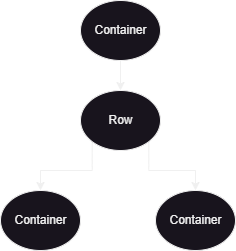
\includegraphics[height=4cm, keepaspectratio]{graphics/widgetTree.png}
    \caption{Voorbeeld van een widgetboom}
\end{figure}
\\
Elk widget is immutable of onveranderlijk. Wanneer zich een gebeurtenis voordoet, zoals een gebruikersinteractie, veranderen applicaties hun gebruikersinterface door het framework te vertellen om een widget in de hiërarchie te vervangen door een andere. 
Het framework werkt als gevolg de gebruikersinterface efficiënt bij door de ouderwidgets te vergelijken met de nieuwe. Indien er een verandering is aan de nieuwe widget, wordt de oude dan vervangen met de nieuwe widget.

\subsection[Widget rendering]{Widget rendering}
\label{sec:Widget rendering}
In de vorige sectie wordt er uitgelegd wat een widget is en dat Flutter een widgetboom heeft. Maar hoe kan flutter widgets efficiënt  widgets kunnen gebouwen? Dit vraag wordt in dit sectie uitgelegd.
\\
Flutter heeft eigenlijk niet enkel 1 boom. Flutter maakt namelijk gebruik van 3 parallel bomen voor het renderen van widgets, die samen bijdragen aan de efficiëntie van een Flutter applicatie. \autocite{adnan2023}
\begin{figure}[h]
    \centering
    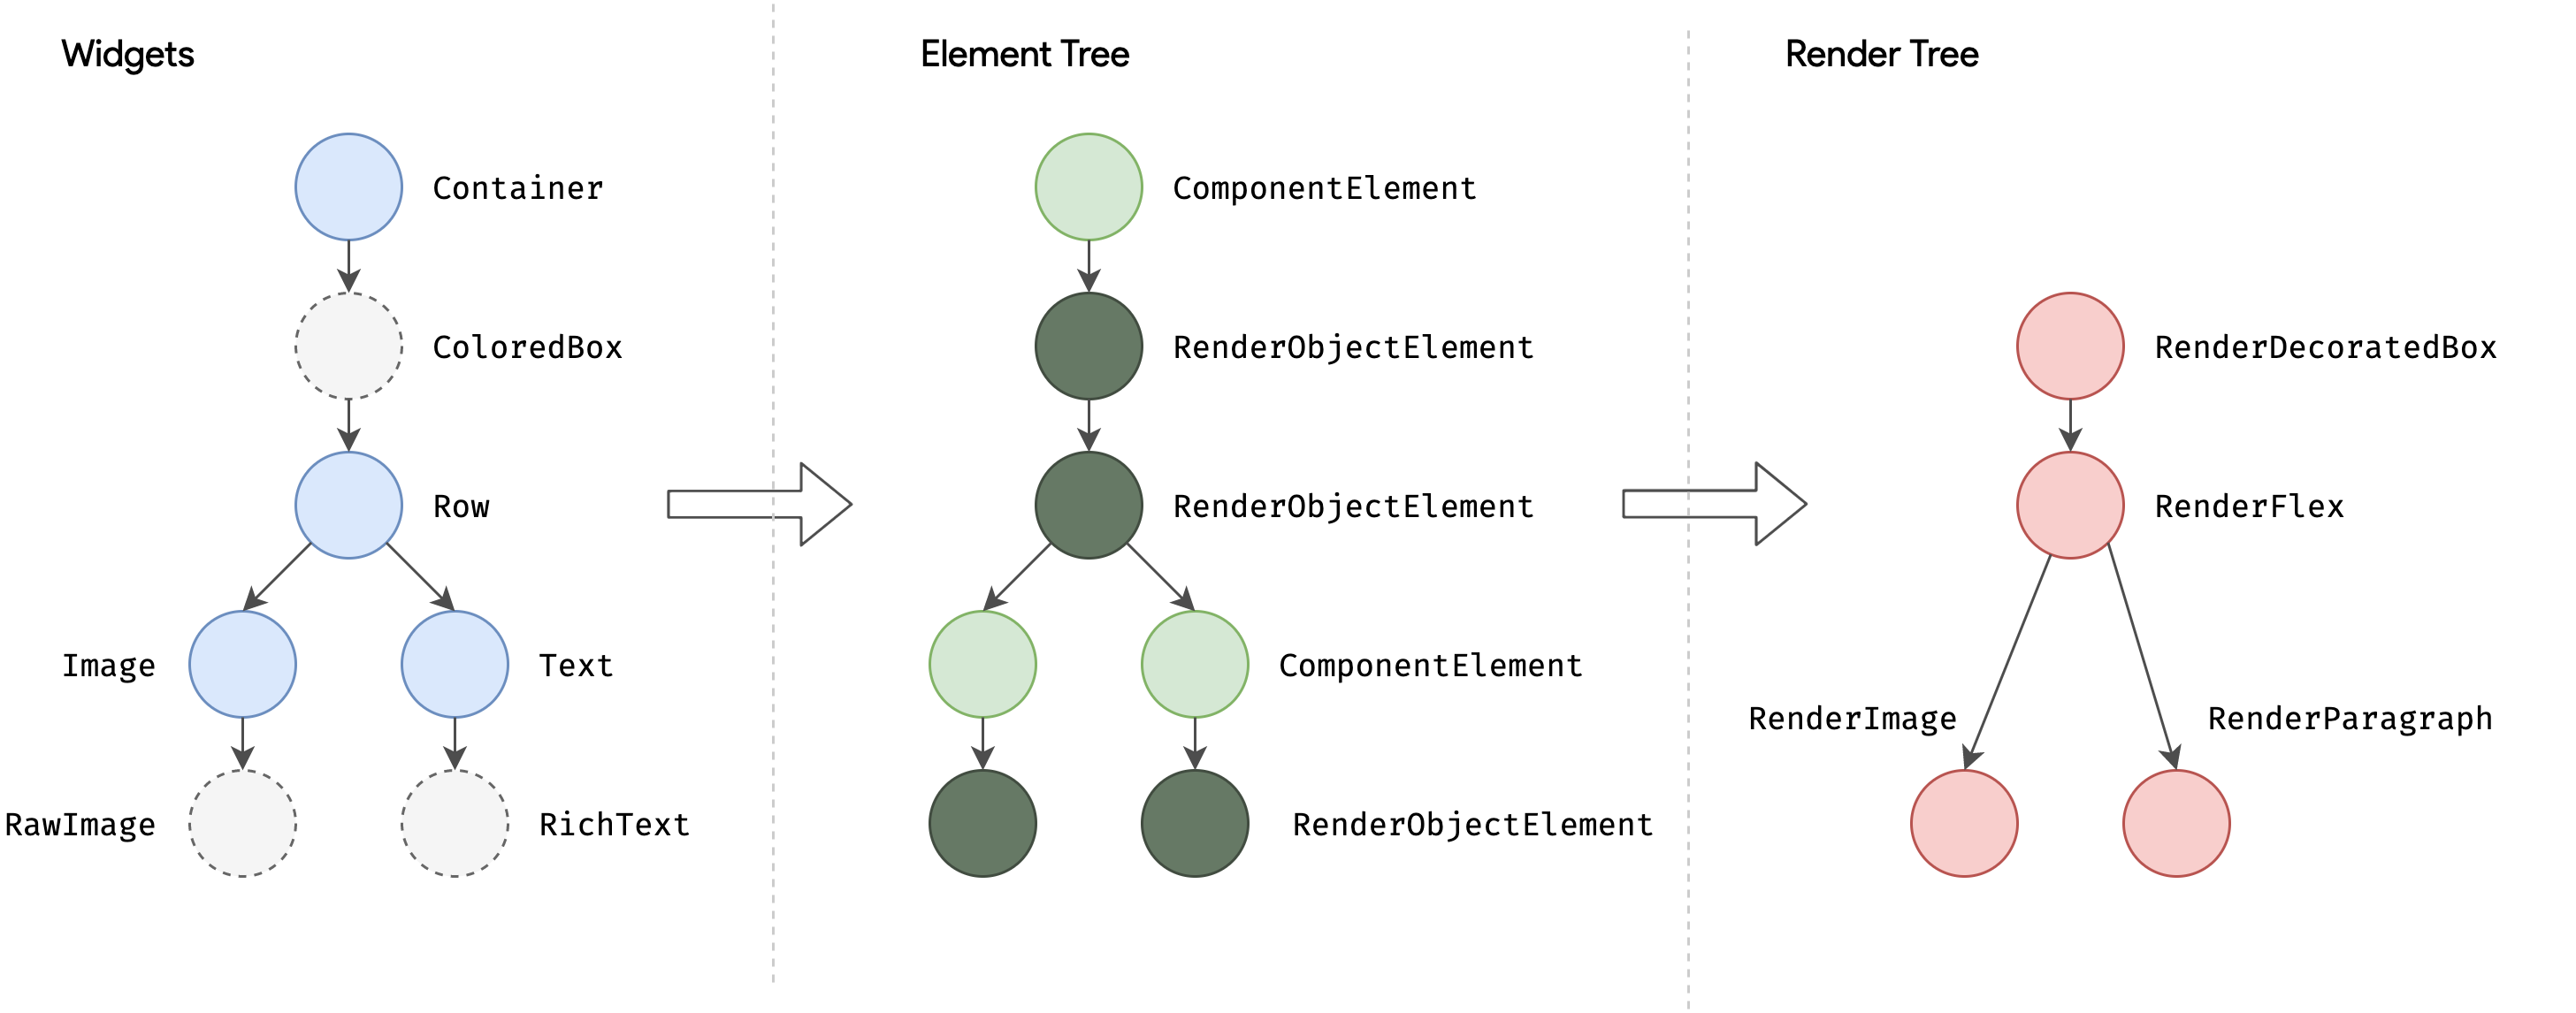
\includegraphics[height=5cm, keepaspectratio]{graphics/trees.png}
    \caption{De 3 widget rendering bomen van Flutter \autocite{flutter2023} }
\end{figure}
\begin{itemize}
    \item \textbf{Widgetboom} 
    \\
    Een widget in een widgetboom vertegenwoordigt de UI-structuur en configuratie.
    \item \textbf{Elementboom} 
   \\
    Tijdens de bouwfase vertaalt Flutter de widgets naar een overeenkomstige elementenboom, met één element voor elke widget. De elementboom beheert updates, wijzigingen van de UI en regelt alles.
   \item \textbf{Renderboom} 
   \\
    Een renderobject in een renderboom is verantwoordelijk voor het finale schilderen van widgets op de User Interface. Het definieert hoe elementen visueel worden weergegeven op het scherm. 
    De renderobject zorgt voor de grootte, lay-out en het schilderen op het scherm. Wat je uiteindelijk op het scherm ziet is geen widget, maar een renderobject.
\end{itemize}



\subsection[states]{States}
\label{sec:States}
Elk widget kan states hebben. Flutter beschrijft een state als informatie die enerzijds synchroon kan worden gelezen wanneer de widget wordt gebouwd en anderzijds
kan veranderen tijdens de levensduur van de widget\footnote{\url{https://api.flutter.dev/flutter/widgets/State-class.html}}. Flutter is declaratief, dit wilt zeggen dat dat Flutter zijn gebruikersinterface bouwt om de huidige status van je app te weerspiegelen.
Indien er een verandering is aan een state, wordt de widget getriggerd en wordt de UI herbouwd.


\subsection[widget states]{Widget states}
\label{sec:Widget states}
Nu dat er een beeld is over wat states zijn binnen Flutter, kan er over de 2 meest gebruikte soorten widgets besproken worden. 
 \begin{itemize}
     \item \textbf{stateless widget} 
     \\
     Stateless widgets, zoals de naam het al zegt, zijn widgets zonder states. Deze widgets worden gedurende de lifecycle van de applicatie niet gewijzigd. Een voorbeeld hiervan is een Icon-widget. Het houdt intern geen states bij en weergeeft altijd een vaste icon.
     \item  \textbf{stateful widget} 
    \\
     Stateful widgets daarentegen kunnen wel state-objecten hebben die kunnen veranderen. Een stateful widget heeft 2 klasse: een klasse van "StatefulWidget" en een klasse "State".
     De state-klasse bevat de veranderbaar state van de widget. Als een widget state wijzijgt door de methode \textit{setState()}  op te roepen, wordt de widget getriggerd om zichzelf te herbouwen en worden alle afstammelingen van deze widget binnen de widgetboom vergeleken met 
     hun oude widget met behulp van de \textit{didWidgetUpdate}-methode en indien er een verandering is worden ze ook herbouwd. 
     \\
     Een voorbeeld van een stateful widget is een Checkbox widget. Indien de user op een checkbox klikt, wordt de state \textit{isChecked} nu gelijk aan \textit{true}. Als gevolg van deze state verandering, wordt de widget opniew gebouwd met een vinkje op de checkbox widget.
\end{itemize}
\begin{figure}[h]
    \centering
    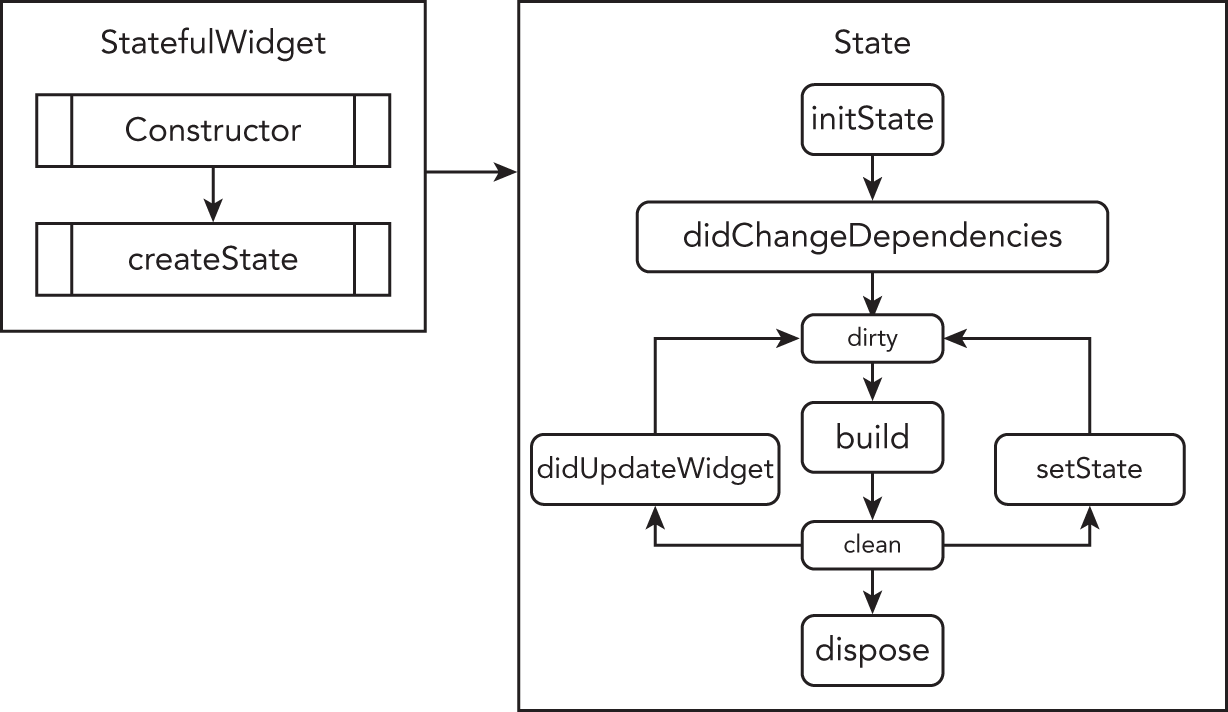
\includegraphics[height=6cm, keepaspectratio]{graphics/widgetLifecycle.png}
    \caption{Lifecycle van een stateless and stateful widget \autocite{Goel2023}}
\end{figure}












\section{{State management}}%
\label{sec:State management}
Zoals eerder vermeld wordt Flutter ontwikkeld om performant te zijn. Maar een mogelijke reden die de performantie van de applicatie kan beïnvloeden is het slecht 
bijhouden van states binnen de applicatie.
\\
State management is een techniek (of meerdere) die gebruikt wordt om veranderingen in de applicatie te beheren. Het gebruik van de juiste state management kan zorgen 
voor betere leesbaarheid van code en ook voor een performanter applicatie. 



\subsection{{setState}}%
\label{sec:setState}
setState is het gemakkelijkste manier om states te veranderen binnen een flutter applicatie. Wanneer de \textit{setState}-method binnen een stateful widget opgeroepen wordt, 
wordt de \textit{build}-method van die widget opgeroepen en wordt het herbouwd met de nieuwe state. Zoals eerder vermeld, als een ouder widget herbouwd wordt, worden er een check gedaan of alle afstammelingen van die ouder herbouwd moeten worden. 
\\
\begin{minted}{dart} 
    class CheckBoxWidget extends StatefulWidget {
  final bool isChecked;
  const CheckBoxWidget({super.key, required this.isChecked});

  @override
  State<CheckBoxWidget> createState() => CheckBoxWidgetState();
}

class CheckBoxWidgetState extends State<CheckBoxWidget> {
  late bool isChecked;
  @override
  void initState() {
    isChecked = widget.isChecked;
    super.initState();
  }

  @override
  Widget build(BuildContext context) {
    return Checkbox(
        value: isChecked,
        onChanged: (value) {
          setState(() {
            isChecked = value!;
          });
        });
  }
}
\end{minted}
\hfill
\\
\textbf{Voor- en nadelen}
\\
Volgens \textcite{slep2020} is het gebruik van setState heel eenvoudig en gemakkelijk te leren, maar er zijn ook wat nadelen aan het gebruik van setState.
\begin{itemize}
    \item Indien een kind diep in de widgetboom een state nodig heeft van een parent aan de top van de boom, moet de state aan alle afstammelingen binnen de widgetboom doorgegeven worden. Dit zorgt voor minder leesbare code en wordt het onderhouden van de code moeilijker.
    \item Er is geen scheiding van views en business logica.
\end{itemize}






\subsection{{Inherited widget}}%
\label{sec:Inherited widget}
Inherited widget lost het probleem op van setState waarbij je properties door de afstammelingen in een widgetboom moet meegeven. Met inherited widget krijgt alle widgets die binnen
de inherited widget subboom zitten toegang tot de inherited widget. Als gevolg hiervan hoeft de properties niet meer aan de kinderen doorgegeven worden, omdat de widgets de properties rechtstreeks kunnen krijgen van de inheritedwidget. \autocite{windmill2020}
\\ 
Als een widget binnen de widgetboom informatie nodig heeft van een inherited widget, kan die widget gebruik maken van de \textit{of}-methode van de inherit widget. Deze methode zoekt in de boomstructuur en vindt de dichtstbijzijnde ouder-inheritedwidget van dat type. 
Een voorbeeld hiervan is als MediaQuery.of(context).size wordt opgeroepen. Flutter zoekt naar de dichstbijzijnde MediaQuery widget, en haalt de size property daarvan. Indien de waarde van de state van de inherited widget wijzigt, worden de consumers van die data dat getroffen is herbouwd.
\\
\begin{minted}{dart} 
class InheritColor extends InheritedWidget {
  const InheritColor({
    super.key,
    required this.color,
    required this.changeColor
    required super.child,
  });

  final Color color;
  final Function(Color color) changeColor;

  static InheritColor of(BuildContext context) {
    final InheritColor? result =
        context.dependOnInheritedWidgetOfExactType<InheritColor>();
    assert(result != null, 'No InheritColor found in context');
    return result!;
  }

  @override
  bool updateShouldNotify(InheritColor oldWidget) => color != oldWidget.color;
}
\end{minted}

Dit is een voorbeeld van hoe je een inherit widget in een stateful widget kan zetten om zijn state te veranderen.  
\begin{minted}{dart}
Color color = Colors.pink;
Widget build(BuildContext context) {
    return InheritColor(
      color: color,
      changeColor: (Color newColor){
        setState(()=>color = newColor);
      },
      child: OtherChildWidget(),
    );
  }
\end{minted}
Wanneer \textit{InheritColor.of(context).changeColor(Colors.green)}  wordt opgeroepen in een widget onder de inheritWidget, zal de \textit{InheritColor}-widget herbouwd worden met een nieuwe Color-object en zullen alle kinderen die luisteren naar de inheritedWidget ook herbouwd worden.
\hfill
\\

\textbf{Voor- en nadelen}
\\
Zoals voordien aangehaald is het grootste pluspunt van inherited widget dat states niet meer door alle constructors moeten indien een state nodig is in een widget op een lage niveau op de widgetboom. 
Een andere voordeel is dat InheritedWidget deel is van de Flutter API, er hoeft dus geen externe package te installeren. 
\\
Een nadeel van inherited widget is dat het geen stand alone state management benadering is. Het is afhankelijk 
van een stateful widget en zijn setstate methode om states van een inherited widget te wijzigen. Er is ook nog altijd boilerplate code nodig: er moet steeds twee klassen zijn: een inheritedWidget en een stateful/stateless widget.




\subsection{{Provider}}%    
\label{sec:Provider}
Provider is de aanbevolen state management benadering volgens de Flutter team. Provider is een wrapper van InheritedWidget om de implementatie ervan gemakkelijker en meer herbruikbaar te maken.
Door de provider te wrappen rond de applicatie, wordt de states van de provider toegankelijk voor alle widgets binnen de applicatie. 
\\
Volgens de documentatie van Provider\footnote{\url{https://pub.dev/packages/provider}} zijn er veel soorten Providers: Provider, ChangeNotifierProvider, ListenableProvider, ProxyProvider, FutureProvider, StreamProvider en veel meer. ChangeNotifierProvider is de provider
die het meest wordt gebruikt.
\\
In de code hieronder wordt een CarModel klasse uitgebreid(extended) met de \textbf{ChangeNotifier}. Een \textit{ChangeNotifier} biedt change notifications(wijzigingemeldingen) aan de luisteraars. Een ChangeNotifier klasse
heeft de methode \textit{notifyListeners}. Dit methode kan opgeroepen worden indien de state wijzigt en een rebuild nodig is in de widget die luistert naar dit state. 
\begin{minted}{dart}
    class CarModel extends ChangeNotifier {
        Color _color = Colors.black;

        Color get color => _color;

        void changeColor(Color newColor) {
             _count = newColor;
            notifyListeners();
        }
}
\end{minted}

\textbf{ChangeNotifierProvider} is een widget die een instantie van ChangeNotifier biedt aan de afstammelingen in de widgetboom.
\begin{minted}{dart}
    Widget build(BuildContext context) {
    return ChangeNotifierProvider(
        create:  (context) => CarModel(),
        child: childWidget(),
    );
  }
\end{minted}
Een \textbf{consumer} is een widget die luistert naar een Provider en geeft het mee aan de widget die het consumeert.
Het is een best practice om je Consumer widgets zo diep mogelijk in de tree te plaatsen. Dit vermijdt dat grote delen van de UI wordt herbouwd omdat ergens een detail is veranderd.

\begin{minted}{dart}
    Widget build(BuildContext context) {
    return Consumer<CarModel>(
        builder: (context, car, child) {
          return Text('The car is ${car.color} in color.');
        },
      );
  }
\end{minted}
Een alternatief voor het Consumer Widget is door context.read<T>() of context.watch<T>() te gebruiken. De watch methode luistert naar de changes van de Provider en triggert een rebuild indien er wijzigingen zijn aan de state van de provider. De read-methode daarentegen
returnt T zonder te luisteren en triggert dus geen rebuilds. Op hetzelfde manier kan er ook gebruikt gemaakt worden van Provider.of<T>(context) om aan de provider te geraken.Er is een optionele parameter listen. Indien de UI niet hoeft te veranderen kan Provider.of<T>(context, listen: false) ook gebruikt worden. 
\hfill
\\ 

\textbf{Voor- en nadelen}
\\
Volgens \textcite{Makadiya2022} is het gebruik van Provider eenvoudiger dan InheritWidget omdat het de boilerplate code vermindert. Bovendien faciliteert het ook de schaalbaarheid van de applicatie.
\\
Een nadeel hiervan is dat provider het onnodig heropbouwen van widgets kan veroorzaken. Als er een verandering is aan een state binnen de Provider, wordt alle widgets die naar dit state luistert 
verwittigd over de verandering en wordt het herbouwt, maar dit hoeft niet altijd te gebeuren.





\subsection{{RiverPod}}%
\label{sec:RiverPod}
Riverpod is een verbetering tegenover de Provider package. Het gebruikt de concepten van Provider en voegt functionaliteiten toe door het verbeteren van flexibiliteit en performantie.\autocite{Arsha2021} 
Riverpod kan netwerkverzoeken uitvoeren met ingebouwde foutafhandeling en caching, terwijl het automatisch gegevens opnieuw ophaalt als dat nodig is \footnote{\url{https://riverpod.dev/docs/introduction/why_riverpod}}.
\\
Om Riverpod te kunnen gebruiken moet er eerste een ProviderScope widget gewrapd worden rond de wortelwidget(rootwidget) van de widgeboom. Deze provider scope houdt alle providers bij en zorgt ervoor dat er geen lek is van de states ondanks dat de providers globaal worden gedeclareerd.
\begin{minted}{dart}
    void main() {
  runApp(
    ProviderScope(
      child: MyApp(),
    ),
  );
}
\end{minted}
De provider van Riverpod zitten buiten de widgetboom. Om die providers te kunnen lezen is er nood aan een extra referentie-object. 
De eerste manier om de data van een provider te lezen is met behulp van een \textit{ConsumerWidget}. In plaats van een widget uit te breiden(extend) met een StatelessWidget, 
wordt een ConsumerWidget gebruikt omdat die een extra Ref object heeft die kan gebruikt worden om naar de providers te luisteren. Voor StatefulWidgets wordt er dan gebruik
gemaakt van een \textit{ConsumerStatefulWidget} en een \textit{ConsumerState}.
\begin{minted}{dart}
    final CarProvider = Provider<String>((_) => 'This is a car');
    class CarWidget extends ConsumerWidget {
        @override
        Widget build(BuildContext context, WidgetRef ref) {
          final car = ref.watch(CarProvider);
          return Text(car);
        }
      }
\end{minted}
Een tweede manier is om een widget te wrappen in een \textit{Consumer}-widget zoals bij de Provider library. Zoals bij de eerste manier is er bij deze ook een Ref-object nodig. In dit geval is de 
Ref object een argument in de builder.
\begin{minted}{dart}
    final CarProvider = Provider<String>((_) => 'This is a car');
    
class CarWidget extends StatelessWidget {
  @override
  Widget build(BuildContext context) {
   
    return Consumer(
      builder: (_, WidgetRef ref, __) {
        return Text(ref.watch(CarProvider));
      },
    );
  }
}
\end{minted}

Er zijn zoals bij de Provider library ook veel soorten providers bij RiverPod: 
\begin{itemize}
    \item   Provider wordt gebruikt voor objecten die niet veranderen of niet mutable zijn. 
    \item   StateProvider wordt gebruikt voor simpele state objecten die kunnen veranderen. StateProvider wordt in RiverPod 2.0 niet meer gebruikt en wordt vervangen door Notifier.
    \item   FutureProvider is een provider voor states die mogelijk niet direct beschikbaar is, maar wel op een bepaald moment in de toekomst. Dit is handig voor asynchroon operaties, zoals het ophalen van data van een externe API.
    \item   StreamProvider is handig wanneer er geluisterd moet worden naar een stream van events, zoals de wijzigingen van een databank.
\end{itemize}
\hfill
\\ 
\textbf{Voor- en nadelen}\\
Er zijn veel voordelen aan het gebruik van Riverpod. Er is meer controle over het herbouwen van widgets. Bovendien is het gemakkelijk te gebruiken met weinig boilerplate code. 
Het enige nadeel van Riverpod is dat je een externe library moet installeren. 
 



% \subsection{{GetX}}%
% \label{sec:GetX}
% todo
% \\
\subsection{{Redux}}%
\label{sec:Redux}
Redux is een library gekend door Javascript developers voor het ontwikkelen van webapplicaties. Echter is het ook mogelijk om Redux te gebruiken met Flutter.
Redux is een architectuur met een unidirectionele dataflow. De states worden verzameld in een centraal geplaatste store. De gegevens in deze centrale 
opslag zijn toegankelijk voor elk widget dat de gegevens nodig heeft, zonder dat er door de afstammelingen van de widgets in de boomstructuur hoeft te gaan. \autocite{Jolayemi2021}

Redux heeft 3 fundamentele principes:
\begin{itemize}
    \item \textbf{Single source of truth}: Er is maar één store van informatie in de hele applicatie
    \item \textbf{Immutability}: De state van de applicatie is onveranderlijk en mag enkel gelezen worden. Dit betekent dus dat indien de waarde van een state wijzigt, dat de state 
         vervangen moet worden door een nieuwe state. 
    \item \textbf{Functions should be the state changers}: Veranderingen aan states mogen enkel gebeuren door een functie. Deze functies, genaamd Reducers, zijn de enige entiteit die veranderingen mogen brengen aan de states. 
\end{itemize}

Voordat er meer over Redux beschreven kan worden, moet er eerst een paar kernbegrippen van Redux uitgelegd worden: 
\\
Een \textbf{Store} is een centrale locatie binnen de applicatie die alle states bijhoudt van de applicatie. Een \textbf{Reducer} is een synchrone functie die de store updatet met een nieuwe state. De reducer is ook de enige 
die de state mag veranderen. Een reducer neemt als argument de vorige state en een Action, en geeft een nieuwe state terug. Een \textbf{Action} beschrijft wat er is gebeurt. Een Action is de object die bepaalt wat er met de state moet gebeuren. 
Met behulp van de dispatch methode wordt een Action meegegeven aan de Store, zodat de state aangepast kan worden volgens de meegegeven Action.
Een \textbf{Middleware} is een speciale functie die uitgevoerd wordt voordat de dispatched Action de Store bereikt. Ze worden meestal gebruikt om te luisteren naar Actions en
asynchrone calls uit te voeren, zoals request naar een externe API. Eens dat er een response is, kan een andere Action dispatched worden naar de Reducer. 
\\
\begin{figure}[h]
    \centering
    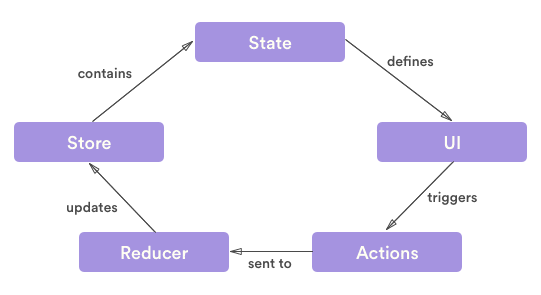
\includegraphics[height=5cm, keepaspectratio]{graphics/reduxcycle.png}
    \caption{Redux lifecycle \autocite{Sharma2018}}
    \label{fig:lifecycle}
\end{figure}
Elk state wijziging in Redux gaat door dezelfde cyclus zoals geïllustreerd in figuure \ref{fig:lifecycle}. 
De UI wordt gedefinieerd door de states. De drie primaire componenten van Redux zijn Store, Reducers en Actions. 
De User interface triggert de Actions, die naar de Reducers worden gestuurd. De Reducers werken vervolgens Stores bij die de states bevatten. 





Met behulp van \textit{StoreProvider}-widget worden alle widgets binnen de widgetboom geinjecteerd met de Redux Store. 
De StoreBuilder-widget geeft de store door aan zijn kind en luistert continue naar de Store. Indien de Store geüpdatet wordt, zal dit het herbouwen van zijn afstammelingen triggeren.
Een alternatief is de \textit{StoreConnector}-widget. De StoreConnector zet de Store om in een ViewModel. Dit is veel performanter omdat het naar de ViewModel luistert. De afstammelingen worden enkel herbouwt als de ViewModel wijzigt.

\begin{minted}{dart}
    class MyApp extends StatelessWidget {
    final store = Store(reducer,
        initialState: AppState.initialState(),
        );

    @override
    Widget build(BuildContext context) {
      return StoreProvider(
        store: store,
        child: MaterialApp(
          title: 'Flutter Redux Demo',
          theme: ThemeData(
            primarySwatch: Colors.blue,
          ),
          home: StoreConnector<int, Model>(
            distinct: true
            converter: (store)=> store.state.toString(),
            builder: ( context,  model) {
                return Text(model.value)
       },
        ),
      ));
    }
  }
\end{minted}

\hfill
\\ 
\textbf{Voor- en nadelen}
\\
Er zijn veel voordelen aan het gebruik van Redux. Redux is ontworpen om bugs te voorkomen door State onveranderlijk te maken en met de unidirectionele dataflow. Ook worden de vorige 5 states bijgehouden, dus indien er iets misloopt wordt het debuggen gemakkelijker. 
\\
De nadelen van Redux is dat er heel veel boilerplate code is. Hoewel het goed is voor synchroon operaties, wordt het wat gecompliceerd bij asynchroon operaties. 
 


\subsection{{Bloc}}%
\label{sec:Bloc}
BLoC staat voor Business Logic Component. Het scheidt de presentatielaag van de business logica, die de code sneller, gemakkelijker om te testen en herbruikbaar maakt.
\begin{figure}[h]
    \centering
    
\includegraphics[height=3cm, keepaspectratio]{graphics/blocArchitectuur.png}
    \caption{BLoC Architectuur \autocite{bloc2023}}
    \label{fig:bloc}
\end{figure}
Door gebruik te maken van BLoC wordt de applicatie verdeeld in 3 lagen \autocite[bloc2023]:
\begin{itemize}
    \item \textbf{Presentatielaag (user interface)} \\
    De verantwoordelijkheid van de presentatielaag is om uit te zoeken hoe hij zichzelf moet renderen op basis van een of meer BLoC-states.
    \item \textbf{Business logica (BLoC)} \\
    De businesslaag is verantwoordelijk voor het reageren op input van de presentatielaag met nieuwe states. Deze laag kan afhankelijk zijn van een of meer repositories om gegevens op te halen die nodig zijn om de states van de applicatie op te bouwen.
    De businesslaag wordt op de hoogte gebracht van gebeurtenissen/acties van de presentatielaag en communiceert vervolgens met de repository om een nieuwe state op te bouwen die de presentatielaag kan gebruiken.
    \item \textbf{Datalaag} \\
    Dit bestaat uit een repository en een data provider. De data provider is een klasse met methoden om CRUD operaties uit te voeren via een (externe) API. De repository is een wrapper
    rond één of meerder data providers en communiceert met de BLoC laag. 
\end{itemize}

\hfill
\\
\textbf{Voor- en nadelen}
Volgens \textcite{slep2020} zijn er veel voordelen voor het gebruik van BLoC:
\begin{itemize}
    \item Het biedt een goeie schaalbaarheid en testbaarheid
    \item  Er is een goed seperation of concerns omdat de business logica in een aparte klasse zit
    \item Het is performant voor groot applicaties
\end{itemize}

De nadelen zijn:
\begin{itemize}
    \item Streams moet in beide richtingen gebruikt worden. Dit leidt tot meer boilerplate code
    \item Het is enkel efficient bij groot applicaties. 
\end{itemize}

% \subsection{{MobX}}%
% \label{sec:MobX}
% todo

% Tip: Begin elk hoofdstuk met een paragraaf inleiding die beschrijft hoe
% dit hoofdstuk past binnen het geheel van de bachelorproef. Geef in het
% bijzonder aan wat de link is met het vorige en volgende hoofdstuk.

% Pas na deze inleidende paragraaf komt de eerste sectiehoofding.

%Dit hoofdstuk bevat je literatuurstudie. De inhoud gaat verder op de inleiding, maar zal het onderwerp van de bachelorproef *diepgaand* uitspitten. De bedoeling is dat de lezer na lezing van dit hoofdstuk helemaal op de hoogte is van de huidige stand van zaken (state-of-the-art) in het onderzoeksdomein. Iemand die niet vertrouwd is met het onderwerp, weet nu voldoende om de rest van het verhaal te kunnen volgen, zonder dat die er nog andere informatie moet over opzoeken \autocite{Pollefliet2011}.

%Je verwijst bij elke bewering die je doet, vakterm die je introduceert, enz.\ naar je bronnen. In \LaTeX{} kan dat met het commando \texttt{$\backslash${textcite\{\}}} of \texttt{$\backslash${autocite\{\}}}. Als argument van het commando geef je de ``sleutel'' van een ``record'' in een bibliografische databank in het Bib\LaTeX{}-formaat (een tekstbestand). Als je expliciet naar de auteur verwijst in de zin (narratieve referentie), gebruik je \texttt{$\backslash${}textcite\{\}}. Soms is de auteursnaam niet expliciet een onderdeel van de zin, dan gebruik je \texttt{$\backslash${}autocite\{\}} (referentie tussen haakjes). Dit gebruik je bv.~bij een citaat, of om in het bijschrift van een overgenomen afbeelding, broncode, tabel, enz. te verwijzen naar de bron. In de volgende paragraaf een voorbeeld van elk.

%\textcite{Knuth1998} schreef een van de standaardwerken over sorteer- en zoekalgoritmen. Experten zijn het erover eens dat cloud computing een interessante opportuniteit vormen, zowel voor gebruikers als voor dienstverleners op vlak van informatietechnologie~\autocite{Creeger2009}.

%Let er ook op: het \texttt{cite}-commando voor de punt, dus binnen de zin. Je verwijst meteen naar een bron in de eerste zin die erop gebaseerd is, dus niet pas op het einde van een paragraaf.


